% chapters/week01.tex
\chapter{The Role of Statistics in Engineering}

\section{Introduction}
We start with two examples from the bachelor \emph{Military Systems and Technology}.

\section{Maintenance: the reliability of a circuit}
Air force helicopters, such as the Apache, rely on complex electronic circuits to operate their avionics and their weapons systems.
One example of such a circuit can be found in the power distribution system.
Critical avionics are often powered by multiple sources independent from each other, in order to increase reliability.
This way, a failure in one power source does not necessarily lead to a failure of the entire system.
Nevertheless, analyzing and predicting the reliability of such circuits is a complex task.

Consider the simple circuit shown in~\cref{fig:circuit}. In this circuit, we have three devices $A$, $B$ and $C$.
In this process, the entire system works properly if the circuit operates.
A circuit operates only if there is a path of functional devices from left to right.
Devices $A$ and $B$ are connected in parallel, while device $C$ is in series with $A$ and $B$.

\begin{figure}[htbp]
  \centering
  % TikZ circuit figure (Figure 1.1)
  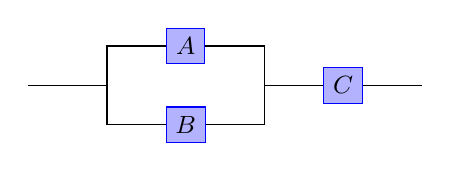
\begin{tikzpicture}[every node/.style={font=\small}]
    % wires
    \draw (0,0) -- (1,0) -- (1, 0.5) -- (3, 0.5) -- (3,0) -- (5,0);
    \draw (0,0) -- (1,0) -- (1, -0.5) -- (3, -0.5) -- (3,0) -- (5,0);
    
    \node[draw=blue, fill=blue!30] at (2, 0.5) {$A$};
    \node[draw=blue, fill=blue!30] at (2, -0.5) {$B$};
    \node[draw=blue, fill=blue!30] at (4, 0) {$C$};
  \end{tikzpicture}
  \caption{Circuit with three devices ($A$ and $B$ in parallel, $C$ in series).}
  \label{fig:circuit}
\end{figure}

For example, the circuit operates if $A$ and $C$ function, but it fails whenever $C$ malfunctions.

Assume now that all devices function on average for $10$ hours.
What is the probability that the circuit will operate for at least $9$ hours?

We look at this problem in two different ways.
First we assume that the device's lifetimes are deterministic, i.e., the lifetimes are always a certain fixed value.
Secondly, we assume that the devices' lifetimes are stochastic, i.e., under influence of randomness or variability.

\begin{itemize}
    \item {\bfseries Deterministic:} each device will function for precisely $10$ hours. In this case, it is easy to see that the entire circuit will also function for precisely $10$ hours.
    \item {\bfseries Stochastic:} each device's lifetime is a randomly chosen value between $5$ and $15$ hours.
    In that case, we need a more elaborate method for computing the probability that the circuit will operate for at least $9$ hours.
    Notice that if we pick a random number between $5$ and $15$, there is a \SI{60}{\percent} probability that the picked value is larger than or equal to $9$ (hours).
    The circuit will function if at least one of $A$ or $B$ functions for at least nine hours \emph{and} $C$ functions for at least nine hours.
    The probability that this will happen is equal to 
    \[
        \left(1 - 0.4 \cdot 0.4\right) \cdot 0.6 = 0.84 \cdot 0.6 = 0.504.
    \]
    In later chapters, we will learn about the general methods to compute such probabilities.
\end{itemize}

\section{Operations Research: Search and Detection}
During World War II, German naval ships used the so-called GIUK-gap (Greenland, Iceland, United Kingdom) to navigate from their bases in Northern Germany to the Atlantic Ocean with the objective of attacking Allied convoys.
However, the Allies had positioned their ships inside the GIUK-gap in order to block the German ships from passing through.
The problem for the Allied ships was to detect the German ships as soon as possible.
To this end, the Allied ships were equipped with radar devices that could detect targets within a certain radius.

This situation of a blocking barrier can be modelled mathematically in the following way:
Consider a lane of width $D$. In this case, this would be the width of the GIUK-gap or more generally, the barrier that the targets are not supposed to pass through.
An observer (Allied ship) moves through the lane at speed $V$ in a fixed pattern along this barrier.
Once the observer reaches the edge of the lane, it reverses course and continues moving in the opposite direction (see~\cref{fig:lane}).
Any target entering the observer's sweep radius $R$ (radius of the observer's sensors) is detected.
We assume that detection is binary: a German ship passing through the gap is either detected or not.

\begin{figure}[htbp]
  \centering
  % TikZ lane + observer (Figure 1.3)
  \begin{tikzpicture}[scale=0.9, every node/.style={font=\small}]
    
    % lane edges
    \draw (0,0) -- (0,6) node[midway, sloped, above] {left edge};
    \draw (8,0) -- (8,6) node[midway, sloped, below] {right edge};

    % observer horizontal motion
    \draw (0, 0.8) -- (3, 0.8);
    \draw (5, 0.8) -- (8, 0.8);

    % observer sweep circle
    \draw[ultra thick, stealth-stealth] (2, 0.8) -- (6, 0.8) node[scale=2, midway, label={above:observer}] {\faShip} node[pos=0.8, above] {$V$};;

    % bracket for D
    \draw[decorate, decoration={brace, mirror, amplitude=15pt}] (0.1,0.2) -- (7.9,0.2) node[midway, below=20pt] {$D$} ;
    % % target arrows (southwards)
    \foreach \x/\y in {1.5/0.5, 2.5/1.1, 3.5/1.4, 4.5/0.7, 5.5/0.9, 6.5/1.6}
      \draw[-stealth, thick] (\x,5.5) -- (\x,5.5-\y) node[midway,right] {};
    \node at (5.0,5.2) {$U$};
  \end{tikzpicture}
  \caption{Linear barrier (observer reversing course at edges).}
  \label{fig:lane}
\end{figure}

Targets move perpendicularly to the observer, at speed $U$.
The target's speed is assumed to be known, while the target's lateral position is unknown.
We model the lateral position $x$ of the target according to the probability density shown in~\cref{fig:pdf}. 
For example, if $D=20$ nm, the probability the target chooses $x\in[-5,5]$ is $0.25$.

\begin{figure}[htbp]
  \centering
  % TikZ probability function (Figure 1.4) - V-shaped density
  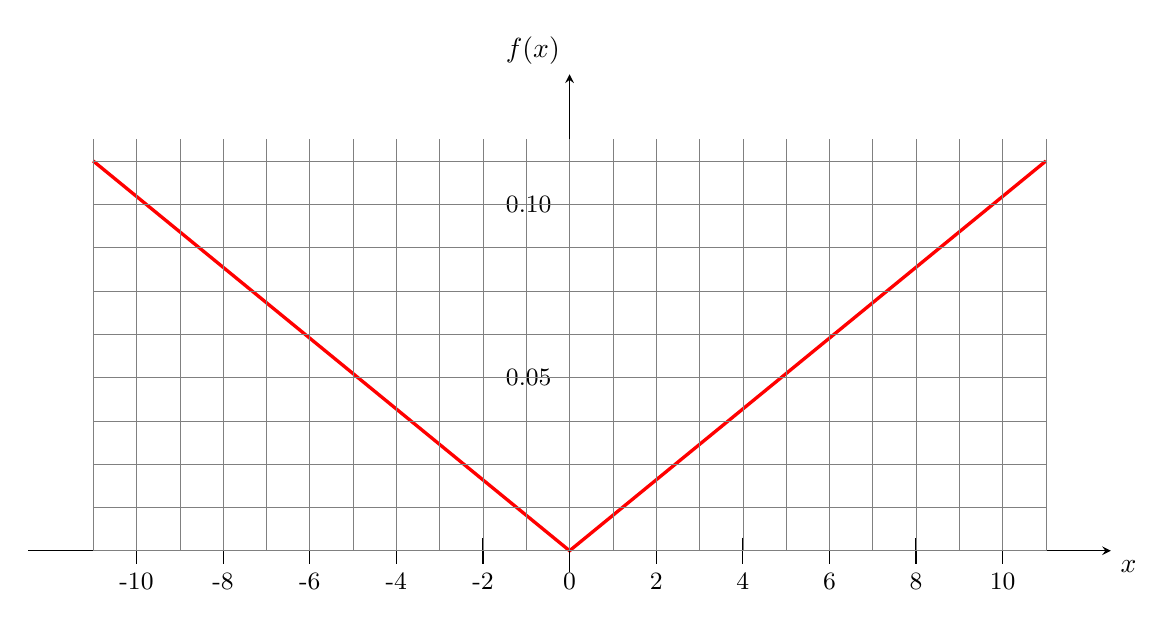
\begin{tikzpicture}[scale=0.55]
    % axes
    \draw[-stealth] (-12.5,0) -- (12.5,0) node[anchor=north west] {$x$};
    \draw[-stealth] (0,-0.5) -- (0,11) node[anchor=south east] {$f(x)$};

    % V-shaped line (symmetric, peak at edges)
    \draw[very thick, red] (-11,9) -- (0,0) -- (11,9);

    % tick marks and labels
    \foreach \x in {-10,-8,-6,-4,-2,0,2,4,6,8,10}
      \draw (\x,0.3) -- (\x,-0.3) node[below,font=\small] {\x};
    \foreach \y/\lab in {4/0.05, 8/0.10}
      \draw (0,\y) node[left=3pt,font=\small] {\(\lab\)};
    \draw[very thin, gray] (-11,0) grid (11,9.5);
  \end{tikzpicture}
  \caption{Probability density function of the lateral position of a target (lane width $D = 20$).}
  \label{fig:pdf}
\end{figure}

Using probability, calculus, and geometry one can derive the following closed-form expression for the detection probability \(P_{\mathrm{det}}\):\\

% === Formula transcribed from PDF ===
\[
    P_{\mathrm{det}} =
    \left[
    \frac{4R^{3}}{3D^{3}}\Bigg(1+\Big(\frac{V}{U}\Big)^{2}\Bigg)
    \;-\;
    \frac{2R^{2}}{D^{2}}\sqrt{\,1+\Big(\frac{V}{U}\Big)^{2}\,} +
    \frac{2R}{D}\right]\cdot \sqrt{\,1+\Big(\frac{V}{U}\Big)^{2}\,}.
\]

% If you prefer a different grouping or an alternate but equivalent algebraic arrangement,
% tell me and I will adjust to match the original typesetting exactly.

\section{Example 1}
For the parameter values shown in the PDF we get the sample computation:

\[
    \begin{aligned}
        D &= 20,\\
        R &= 4,\\
        V &= 18,\\
        U &= 12,
    \end{aligned}
    \qquad\Rightarrow\qquad
    P_{\mathrm{det}} \approx 0.5236.
\]

\section{Exercises}
\begin{enumerate}
  \item Recompute the detection probability for $D = 30$, $R=5$, $V=12$ and $U=10$.
  \item Implement the circuit simulation in Excel or Python, and verify the approximate probability $0.26$ for the device lifetimes used in the PDF.
\end{enumerate}
